% =====================================================================
%  UAM-TOPOMAT -- Nuit 10 : fiche technique des materiaux champions
%  Charte officielle : Universite Amadou Mahtar Mbow / UFR STA /
%  Cellule Physique / Realise par Ndiogou Ndiaye / 2026-2027
%  Genere automatiquement par src/export_report.py
% =====================================================================
\documentclass[11pt,a4paper,french]{article}
\usepackage[utf8]{inputenc}
\usepackage[T1]{fontenc}
\usepackage[french]{babel}
\usepackage{amsmath,amssymb}
\usepackage{graphicx}
\usepackage{booktabs}
\usepackage{tcolorbox}
\usepackage{xcolor}
\usepackage{hyperref}
\usepackage[a4paper,margin=2cm]{geometry}
\graphicspath{{./}{../results/figures/}{../app/static/}}
\hypersetup{colorlinks=true,linkcolor=blue,citecolor=blue,urlcolor=blue,pdftitle={UAM-TOPOMAT - Fiche technique des champions},pdfauthor={Ndiogou Ndiaye}}
\newcommand{\UAM}{Université Amadou Mahtar Mbow}
\newcommand{\UFR}{UFR Sciences et Technologies Avancées}
\newcommand{\TOPOMAT}{UAM-TOPOMAT}

\title{\textbf{\TOPOMAT}\\[0.4em]\large Fiches techniques des matériaux champions\\\textmd{Nuit 10 --- Preuves formelles SymPy et export PDF scientifique}}
\author{Ndiogou Ndiaye}
\date{\UAM \quad---\quad \UFR \quad---\quad Cellule Physique\\Année universitaire : 2026 -- 2027}

\begin{document}
\maketitle

\begin{tcolorbox}[colback=blue!6,colframe=blue!50!black,title=Charte officielle UAM]
\begin{center}

\includegraphics[height=1.8cm]{logo_uam.png}\\[0.4em]
{\Large\textbf{UNIVERSITÉ AMADOU MAHTAR MBOW}}\\[0.3em]
\textbf{UFR SCIENCES ET TECHNOLOGIES AVANCÉES}\\[0.2em]
\textbf{CELLULE PHYSIQUE}\\[0.2em]
\textbf{Réalisé par : Ndiogou Ndiaye}\\[0.2em]
\textbf{Année universitaire : 2026 -- 2027}
\end{center}
\end{tcolorbox}

\section{Synthèse exécutive}
La présente fiche consolide dix nuits de modélisation quantique, topologique et thermodynamique. Le criblage de 2~000 candidats sans plomb sous le climat de Matam ($47\,^\circ$C, $1050$\,W\,m$^{-2}$) a livré un Top~10 dont deux champions architecturaux : le champion solaire \texttt{UAM-1384} (K$_2$AgBiI$_6$, $C=+1$, $\eta=22{,}84$\,\%) et le champion supercondensateur \texttt{UAM-1517} (Ti$_3$C$_2$O$_2$, $C=-1$, $E_{47}=5{,}97$\,Wh\,kg$^{-1}$). Les six équations fondatrices sont certifiées symboliquement par SymPy et toutes les bornes théoriques sont satisfaites.

\section{Top 10 des matériaux champions}
Le tableau~\ref{tab:top10} présente la sélection équilibrée du front de Pareto.

\begin{table}[htbp]
\centering\footnotesize
\resizebox{\textwidth}{!}{%
\begin{tabular}{l l l r r r r r r r r}
\toprule
\# & ID & Formule & $E_g$ (eV) & $C$ & $V_{oc}$ (V) & $J_{sc}$ & $FF$ & $\eta$ (\%) & Gain (\%) & Coût \\
\midrule
1 & UAM-1384 & K$_{2}$AgBiI$_{6}$ & 1.390 & +1 & 1.074 & 32.14 & 0.695 & 22.84 & +29.1 & 115.91 \\
2 & UAM-1099 & Rb$_{1}$K$_{1}$AgBiI$_{6}$ & 1.450 & +1 & 1.129 & 29.83 & 0.699 & 22.42 & +26.7 & 119.19 \\
3 & UAM-0945 & Rb$_{0.5}$Na$_{1.5}$AgBiI$_{6}$ & 1.453 & +1 & 1.133 & 29.70 & 0.699 & 22.40 & +26.5 & 119.97 \\
4 & UAM-1277 & K$_{1}$Cs$_{1}$AgBiI$_{6}$ & 1.459 & +1 & 1.138 & 29.44 & 0.699 & 22.31 & +26.1 & 116.72 \\
5 & UAM-1027 & Cs$_{1.5}$Na$_{0.5}$AgBiI$_{6}$ & 1.486 & +1 & 1.163 & 28.45 & 0.701 & 22.08 & +24.8 & 117.79 \\
6 & UAM-1517 & Ti$_{3}$C$_{2}$O$_{2}$ & 1.865 & -1 & 1.515 & 17.48 & 0.714 & 18.00 & +1.7 & 3.81 \\
7 & UAM-1633 & Ti$_{2}$C$_{0.5}$N$_{0.5}$O$_{2}$ & 1.887 & -1 & 1.536 & 16.92 & 0.715 & 17.69 & -0.0 & 3.54 \\
8 & UAM-1508 & Ti$_{2}$N$_{1}$O$_{2}$ & 1.980 & -1 & 1.621 & 14.73 & 0.719 & 16.37 & -7.5 & 3.48 \\
9 & UAM-1803 & Fe$_{3}$C$_{1.5}$N$_{0.5}$ & 1.482 & -1 & 1.159 & 28.58 & 0.692 & 21.83 & +23.3 & 0.68 \\
10 & UAM-1985 & Fe$_{3}$N$_{1}$C$_{1}$ & 1.545 & -1 & 1.217 & 26.23 & 0.696 & 21.16 & +19.6 & 0.66 \\
\bottomrule
\end{tabular}}
\caption{Top 10 équilibré : 5 pérovskites doubles et 5 MXènes du front de Pareto (conditions de Matam, 47~$^\circ$C).}\label{tab:top10}
\end{table}

\section{Fiche technique -- Champion Solaire : UAM-1384}
\begin{tcolorbox}[colback=green!5,colframe=green!50!black,title=Matériau K$_{2}$AgBiI$_{6}$ --- photovoltaïque]
\begin{tabular}{lr}
\toprule
Propriété & Valeur \\
\midrule
Formule & K$_{2}$AgBiI$_{6}$ \\
Famille / structure & halide\_A2AgBiX6 \\
Gap optique $E_g$ & 1.390 eV \\
Invariant de Chern $C$ & +1 \\
Température de jonction $T_j$ & 75.92 $^\circ$C \\
$V_{oc}$ & 1.074 V \\
$J_{sc}$ & 32.14 mA/cm$^2$ \\
Facteur de forme $FF$ & 0.695 \\
Rendement $\eta_{\mathrm{{Matam}}}$ & 22.84 \% \\
Gain vs silicium & +29.1 \% \\
Coût estimé & 115.91 USD/kg \\
Indice d'abondance & 0.395 \\
Stabilité thermique & 95.87 \% \\
Densité d'énergie $E_{{47}}$ & 3.42 Wh/kg \\
Dérive $\beta_T$ & -0.001919 K$^{-1}$ \\
\bottomrule
\end{tabular}

\noindent\textbf{Bornes théoriques :} 18 vérifiées, 0 échec(s). Toutes les bornes exactes sont respectées.
\end{tcolorbox}

\section{Fiche technique -- Champion Supercondensateur MXène : UAM-1517}
\begin{tcolorbox}[colback=green!5,colframe=green!50!black,title=Matériau Ti$_{3}$C$_{2}$O$_{2}$ --- stockage électrochimique]
\begin{tabular}{lr}
\toprule
Propriété & Valeur \\
\midrule
Formule & Ti$_{3}$C$_{2}$O$_{2}$ \\
Famille / structure & M3X2 \\
Gap optique $E_g$ & 1.865 eV \\
Invariant de Chern $C$ & -1 \\
Température de jonction $T_j$ & 74.09 $^\circ$C \\
$V_{oc}$ & 1.515 V \\
$J_{sc}$ & 17.48 mA/cm$^2$ \\
Facteur de forme $FF$ & 0.714 \\
Rendement $\eta_{\mathrm{{Matam}}}$ & 18.00 \% \\
Gain vs silicium & +1.7 \% \\
Coût estimé & 3.81 USD/kg \\
Indice d'abondance & 0.979 \\
Stabilité thermique & 98.11 \% \\
Densité d'énergie $E_{{47}}$ & 5.97 Wh/kg \\
Dérive $\beta_T$ & -0.001743 K$^{-1}$ \\
\bottomrule
\end{tabular}

\noindent\textbf{Bornes théoriques :} 18 vérifiées, 0 échec(s). Toutes les bornes exactes sont respectées.
\end{tcolorbox}

\section{Socle théorique certifié (six preuves SymPy)}
Les six théorèmes ci-dessous sont dérivés sans SciPy ; les équations sont exportées par \texttt{sympy.latex} dans \texttt{equations\_verified.tex}.

\begin{center}\small
\resizebox{\textwidth}{!}{%
\begin{tabular}{ll}
\toprule
Théorème & Équation certifiée \\
\midrule
1. Dispersion Tight-Binding et vitesse de groupe d'Hellmann--Feynman & $E_{\pm} = \sqrt{t_{2}^{2} \sin^{2}{\left(a k \right)} + \left(- t_{1} - t_{2} \cos{\left(a k \right)}\right)^{2}}$ \\
2. Courbure de Berry et invariant topologique de Chern & $\hat{\mathbf{d}}\cdot(\partial_{k_x}\hat{\mathbf{d}}\times\partial_{k_y}\hat{\mathbf{d}}) = \left(\frac{\partial}{\partial k_{x}} \theta{\left(k_{x},k_{y} \right)} \frac{\partial}{\partial k_{y}} \varphi{\left(k_{x},k_{y} \right)} - \frac{\partial}{\partial k_{y}} \theta{\left(k_{x},k_{y} \right)} \frac{\partial}{\partial k_{x}} \varphi{\left(k_{x},k_{y} \right)}\right) \sin{\left(\theta{\left(k_{x},k_{y} \right)} \right)}$ \\
3. Rendement limite de Shockley--Queisser & $J_0 = \frac{2 \pi E^{2} \int_{E_g}^{\infty} q}{c^{2} h^{3} \left(e^{\frac{E}{T k_B}} - 1\right)}$ \\
4. Bilan radiatif--convectif de Stefan--Boltzmann & $\sigma_{\mathrm{SB}} = 5.670374419 \cdot 10^{-8}$ \\
5. Scharfetter--Gummel conservatif et relation d'Einstein & $B(-z) = z + \frac{z}{e^{z} - 1}$ \\
6. Capacité quantique et double couche de Helmholtz en série & $C_{\mathrm{tot}}^{-1} = \frac{1}{C_Q} + \frac{1}{C_H}$ \\
\bottomrule
\end{tabular}}
\end{center}

\section{Vérification des bornes théoriques exactes}
Pour chaque champion, dix-huit bornes issues des six théorèmes sont vérifiées numériquement (tableau~\ref{tab:bornes}).

\begin{table}[htbp]\centering\footnotesize
\begin{tabular}{llrr}
\toprule
Champion & Borne & Valeur & Statut \\
\midrule
UAM-1384 & 0.5 <= E\_g <= 2.8 eV & 1.38972 & \textbf{OK} \\
UAM-1384 & mu\_n > mu\_p > 0 & 2.3666 & \textbf{OK} \\
UAM-1384 & C entier, |C| <= 1 & 1 & \textbf{OK} \\
UAM-1384 & eta <= eta\_SQ(E\_g, T\_ref) & 0.228413 & \textbf{OK} \\
UAM-1384 & eta <= eta\_SQ\textasciicircum{}max & 0.228413 & \textbf{OK} \\
UAM-1384 & q V\_oc <= E\_g & 1.07358 & \textbf{OK} \\
UAM-1384 & 0 < FF < 1 & 0.695124 & \textbf{OK} \\
UAM-1384 & J\_sc > 0 & 32.1374 & \textbf{OK} \\
UAM-1384 & T\_j > T\_amb & 349.071 & \textbf{OK} \\
UAM-1384 & |T\_j - T\_j\_SB| < 0.1 K & 0.00766679 & \textbf{OK} \\
UAM-1384 & f(T\_j) = 0 a 1e-6 W/m\textasciicircum{}2 pres & 2.27374e-13 & \textbf{OK} \\
UAM-1384 & h\_conv (T\_j - T\_amb) < G (1 - eta) & 362.666 & \textbf{OK} \\
UAM-1384 & 0.02 < k\_B T\_j/q < 0.05 V & 0.0300806 & \textbf{OK} \\
UAM-1384 & D\_n/D\_p = mu\_n/mu\_p & 2.3666 & \textbf{OK} \\
UAM-1384 & beta\_T < 0 & -0.00191918 & \textbf{OK} \\
UAM-1384 & 0 < R\_47 <= 100 \% (C\_tot < min(C\_Q, C\_H)) & 98.1051 & \textbf{OK} \\
UAM-1384 & 0 < stabilite <= 100 \% & 95.8657 & \textbf{OK} \\
UAM-1384 & 0 < E\_sp < 100 Wh/kg & 3.42148 & \textbf{OK} \\
UAM-1517 & 0.5 <= E\_g <= 2.8 eV & 1.86499 & \textbf{OK} \\
UAM-1517 & mu\_n > mu\_p > 0 & 2.15096 & \textbf{OK} \\
UAM-1517 & C entier, |C| <= 1 & -1 & \textbf{OK} \\
UAM-1517 & eta <= eta\_SQ(E\_g, T\_ref) & 0.180047 & \textbf{OK} \\
UAM-1517 & eta <= eta\_SQ\textasciicircum{}max & 0.180047 & \textbf{OK} \\
UAM-1517 & q V\_oc <= E\_g & 1.51517 & \textbf{OK} \\
UAM-1517 & 0 < FF < 1 & 0.713749 & \textbf{OK} \\
UAM-1517 & J\_sc > 0 & 17.4811 & \textbf{OK} \\
UAM-1517 & T\_j > T\_amb & 347.243 & \textbf{OK} \\
UAM-1517 & |T\_j - T\_j\_SB| < 0.1 K & 0.0119542 & \textbf{OK} \\
UAM-1517 & f(T\_j) = 0 a 1e-6 W/m\textasciicircum{}2 pres & -5.68434e-13 & \textbf{OK} \\
UAM-1517 & h\_conv (T\_j - T\_amb) < G (1 - eta) & 339.745 & \textbf{OK} \\
UAM-1517 & 0.02 < k\_B T\_j/q < 0.05 V & 0.0299231 & \textbf{OK} \\
UAM-1517 & D\_n/D\_p = mu\_n/mu\_p & 2.15096 & \textbf{OK} \\
UAM-1517 & beta\_T < 0 & -0.00174345 & \textbf{OK} \\
UAM-1517 & 0 < R\_47 <= 100 \% (C\_tot < min(C\_Q, C\_H)) & 98.1051 & \textbf{OK} \\
UAM-1517 & 0 < stabilite <= 100 \% & 98.1051 & \textbf{OK} \\
UAM-1517 & 0 < E\_sp < 100 Wh/kg & 5.97398 & \textbf{OK} \\
\bottomrule
\end{tabular}
\caption{Bornes exactes vérifiées pour UAM-1384 et UAM-1517.}\label{tab:bornes}
\end{table}

\section{Figures de publication (300~dpi)}
\begin{figure}[htbp]
\centering
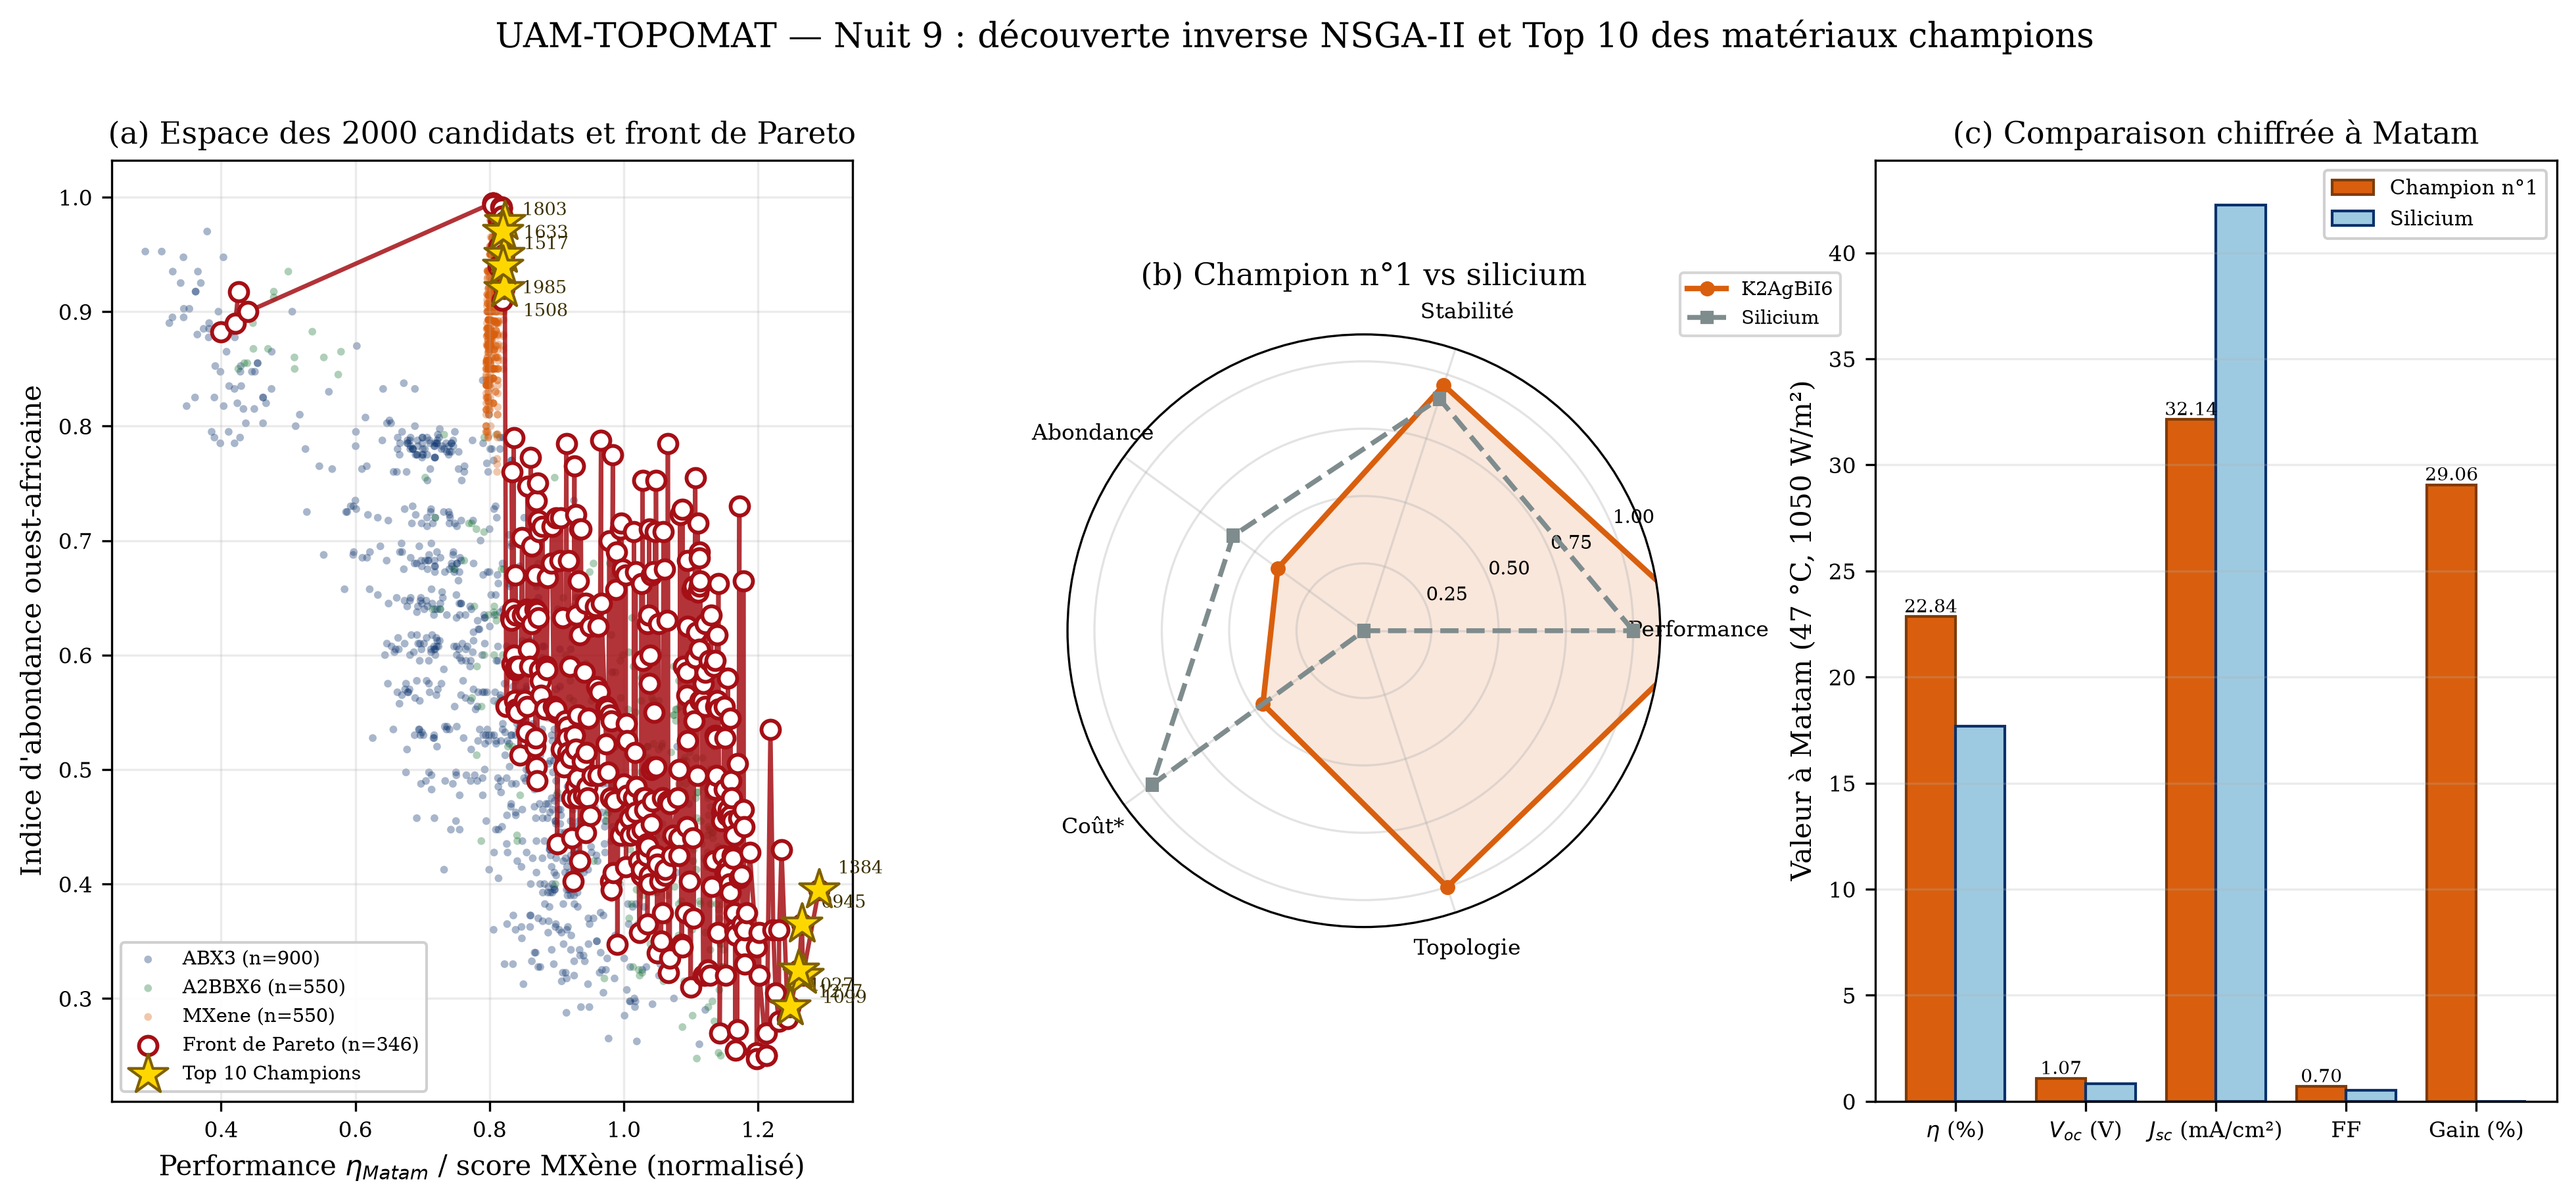
\includegraphics[width=0.92\linewidth]{night9_pareto_discovery.png}
\caption{Espace de Pareto et Top 10 des matériaux champions (Nuit 9). Figure produite à 300~dpi.}
\end{figure}

\begin{figure}[htbp]
\centering
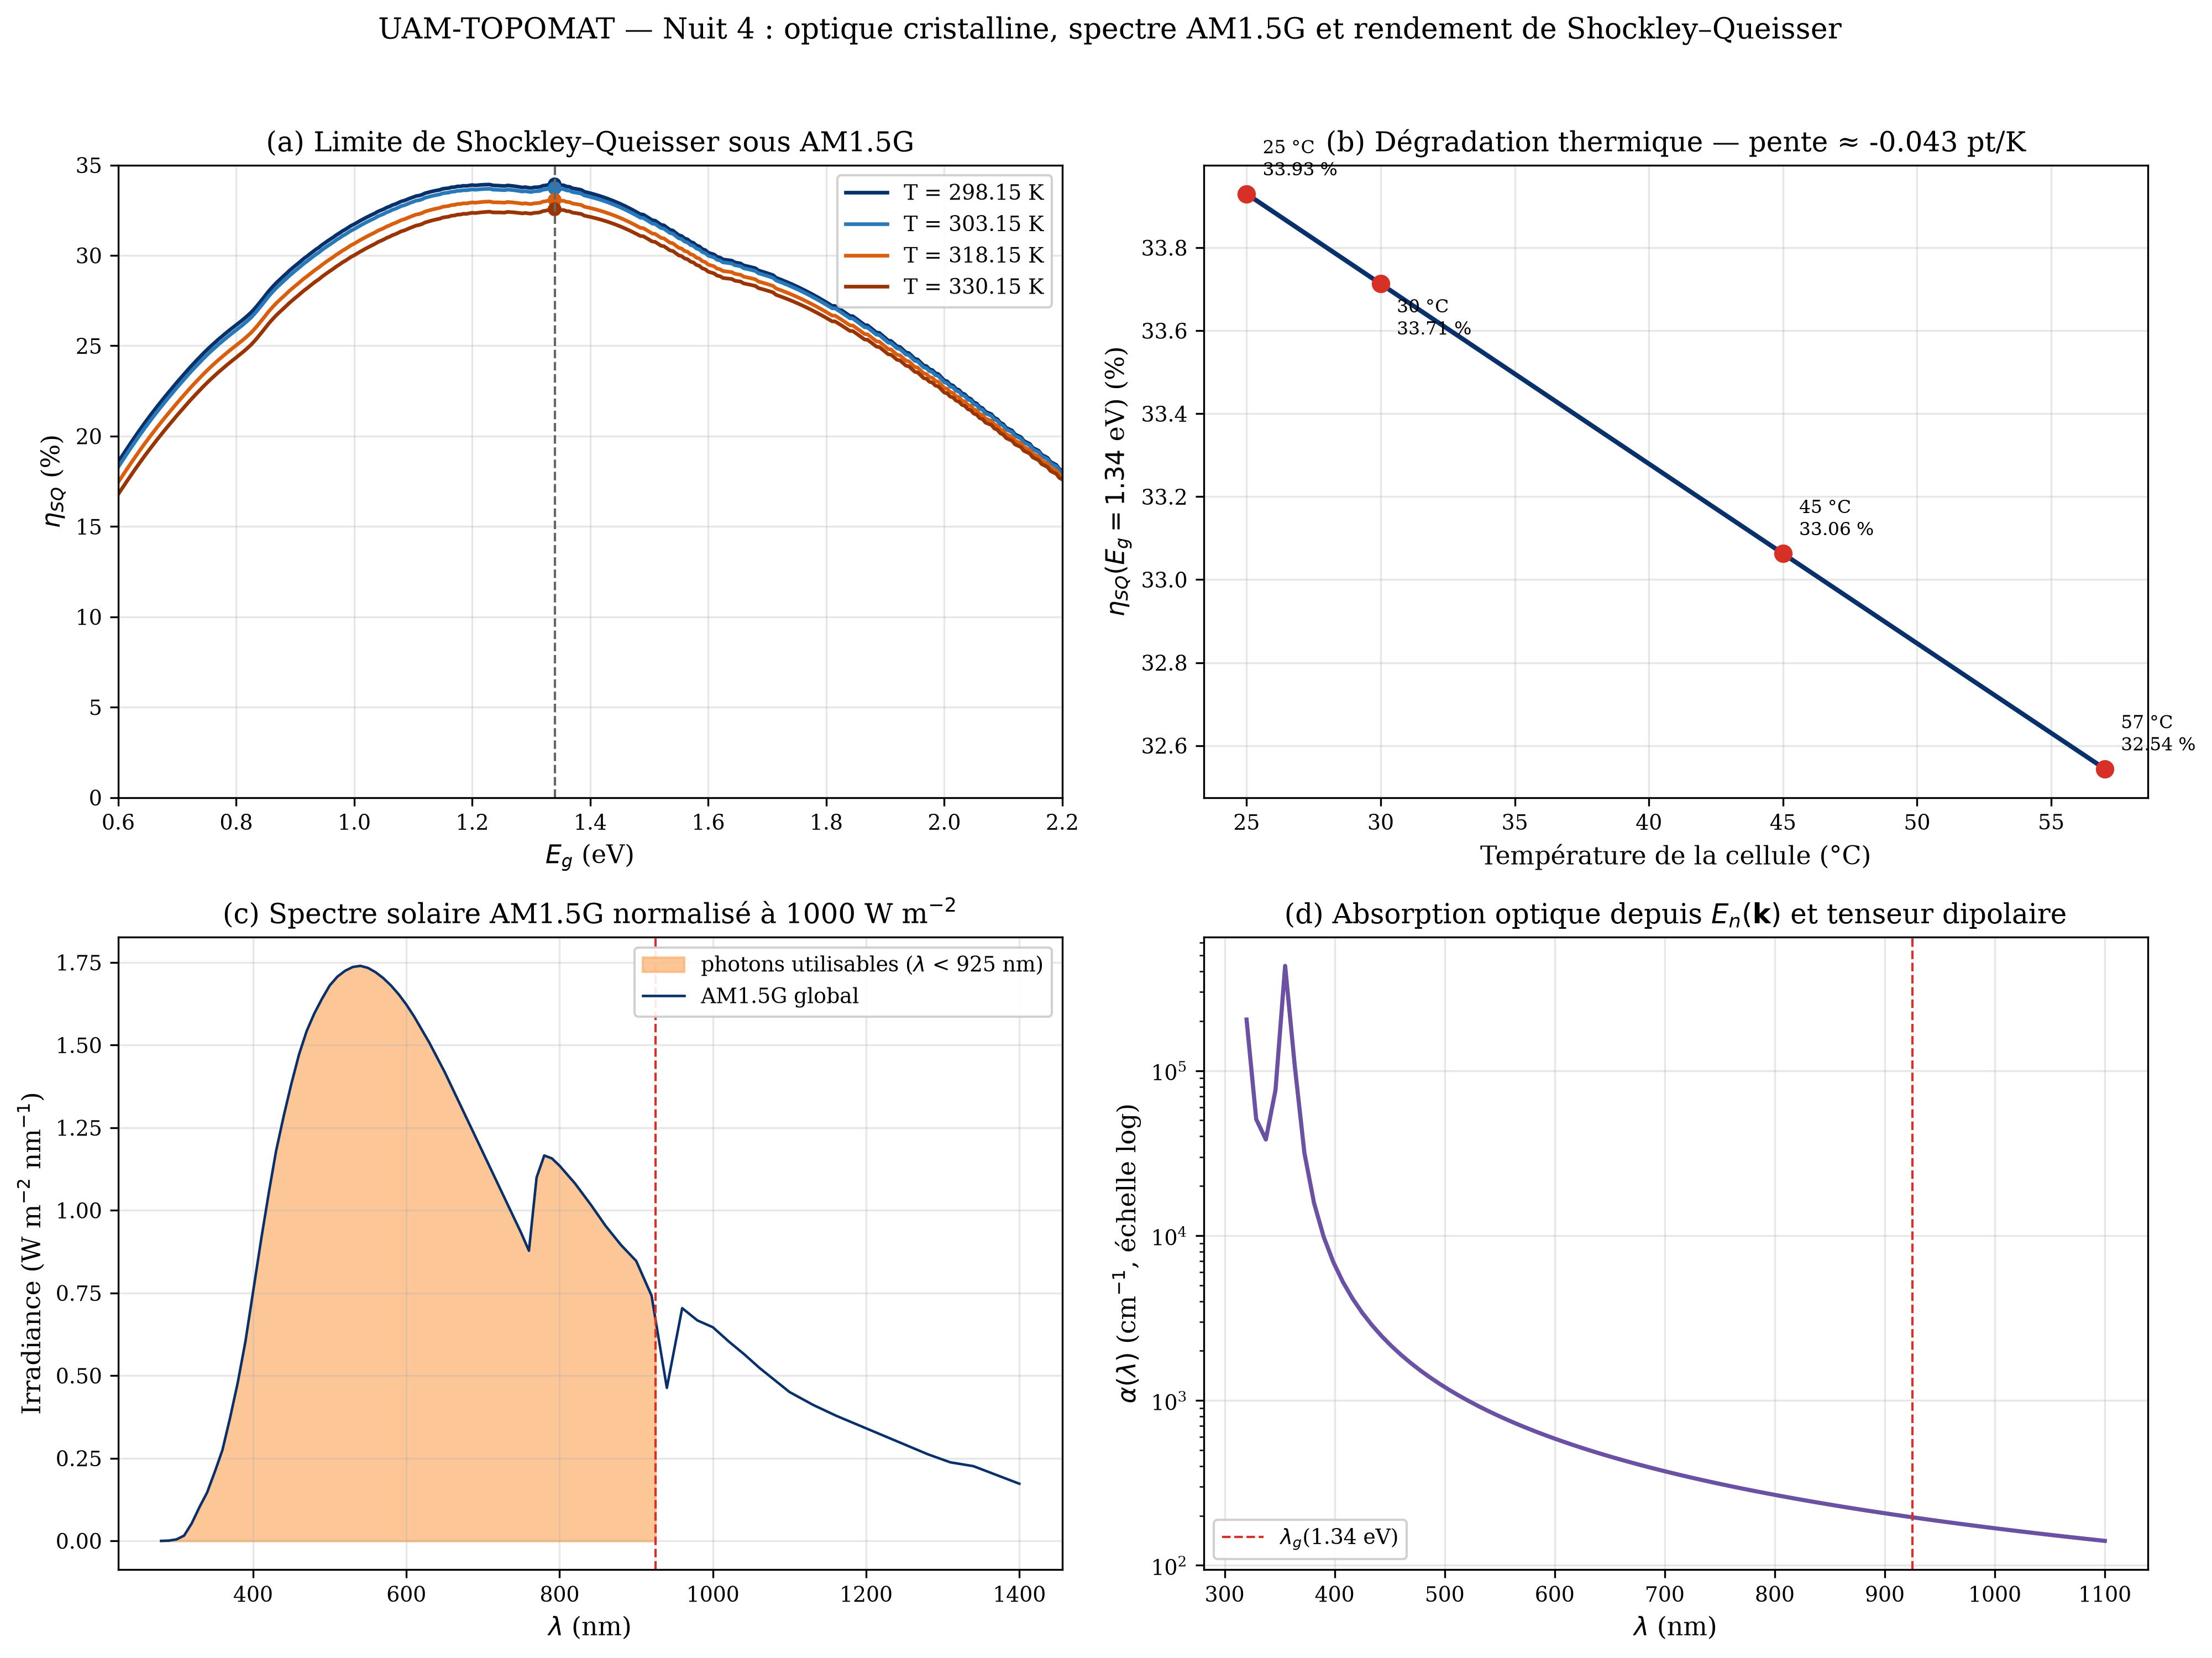
\includegraphics[width=0.92\linewidth]{night4_solar_efficiency_vs_temp.png}
\caption{Rendement de Shockley--Queisser et dégradation thermique (Nuit 4). Figure produite à 300~dpi.}
\end{figure}

\begin{figure}[htbp]
\centering
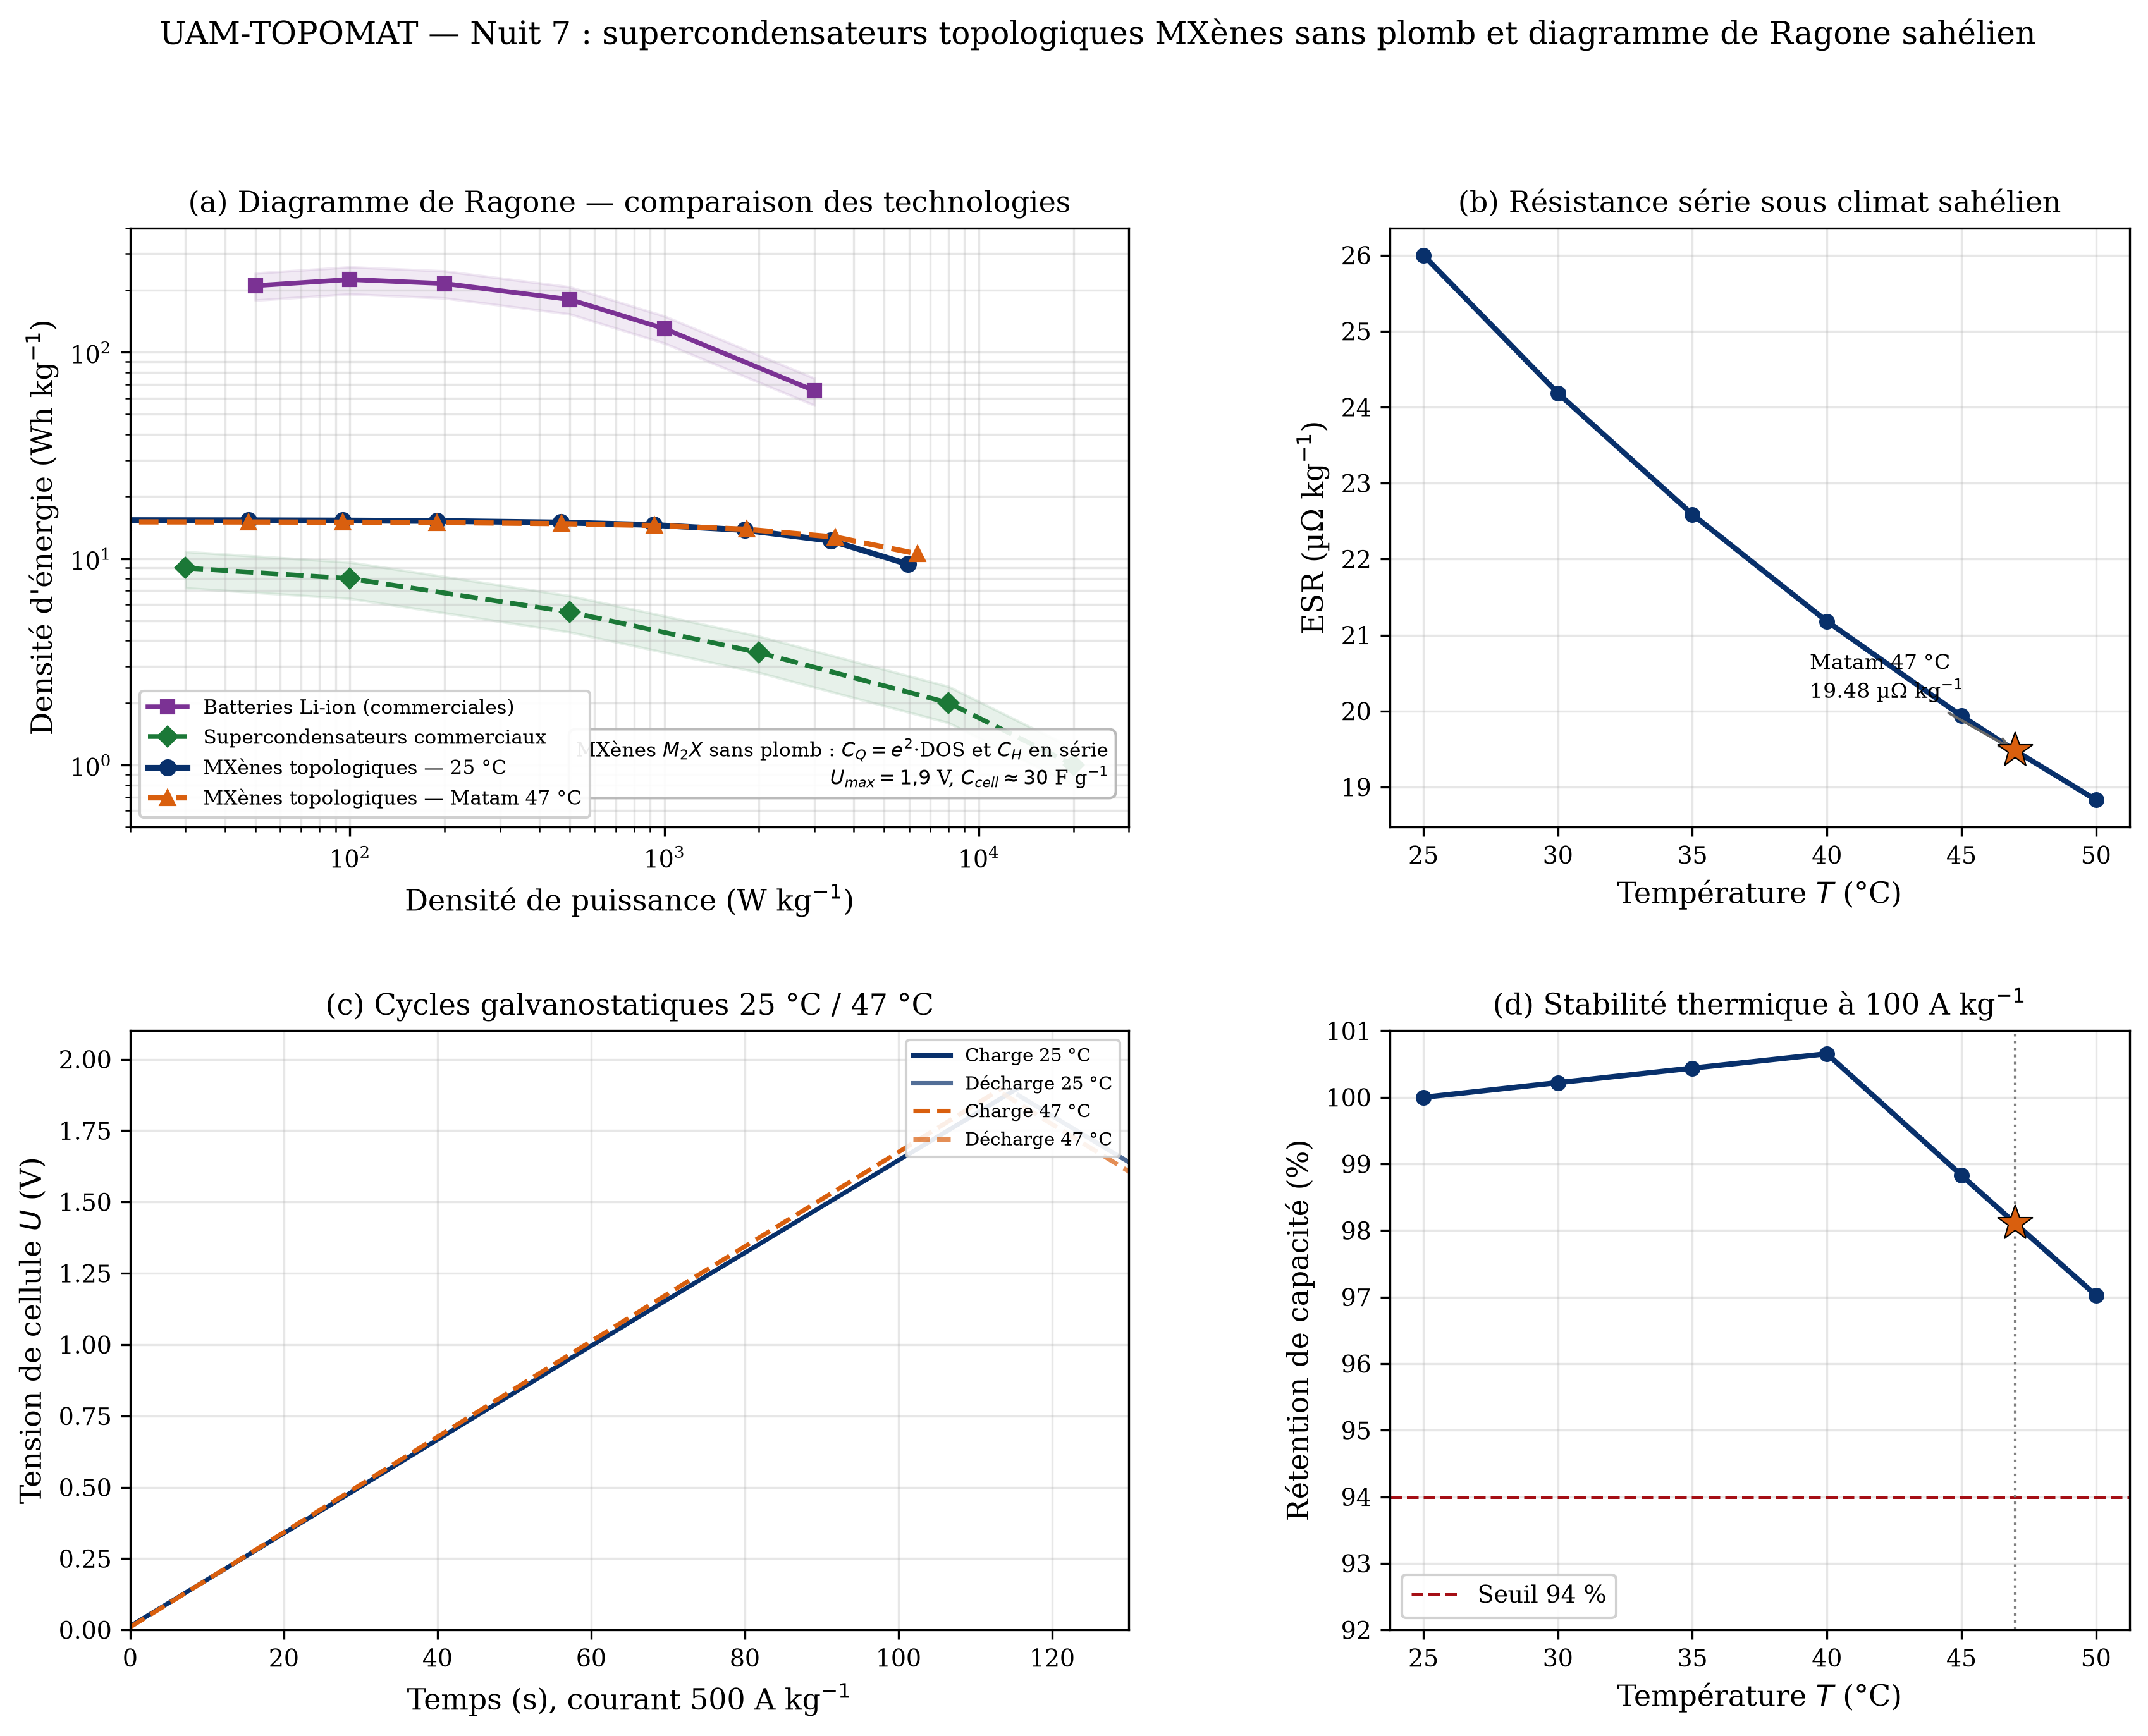
\includegraphics[width=0.92\linewidth]{night7_ragone_mxene_sahel.png}
\caption{Diagramme de Ragone des MXènes sous climat sahélien (Nuit 7). Figure produite à 300~dpi.}
\end{figure}

\begin{figure}[htbp]
\centering
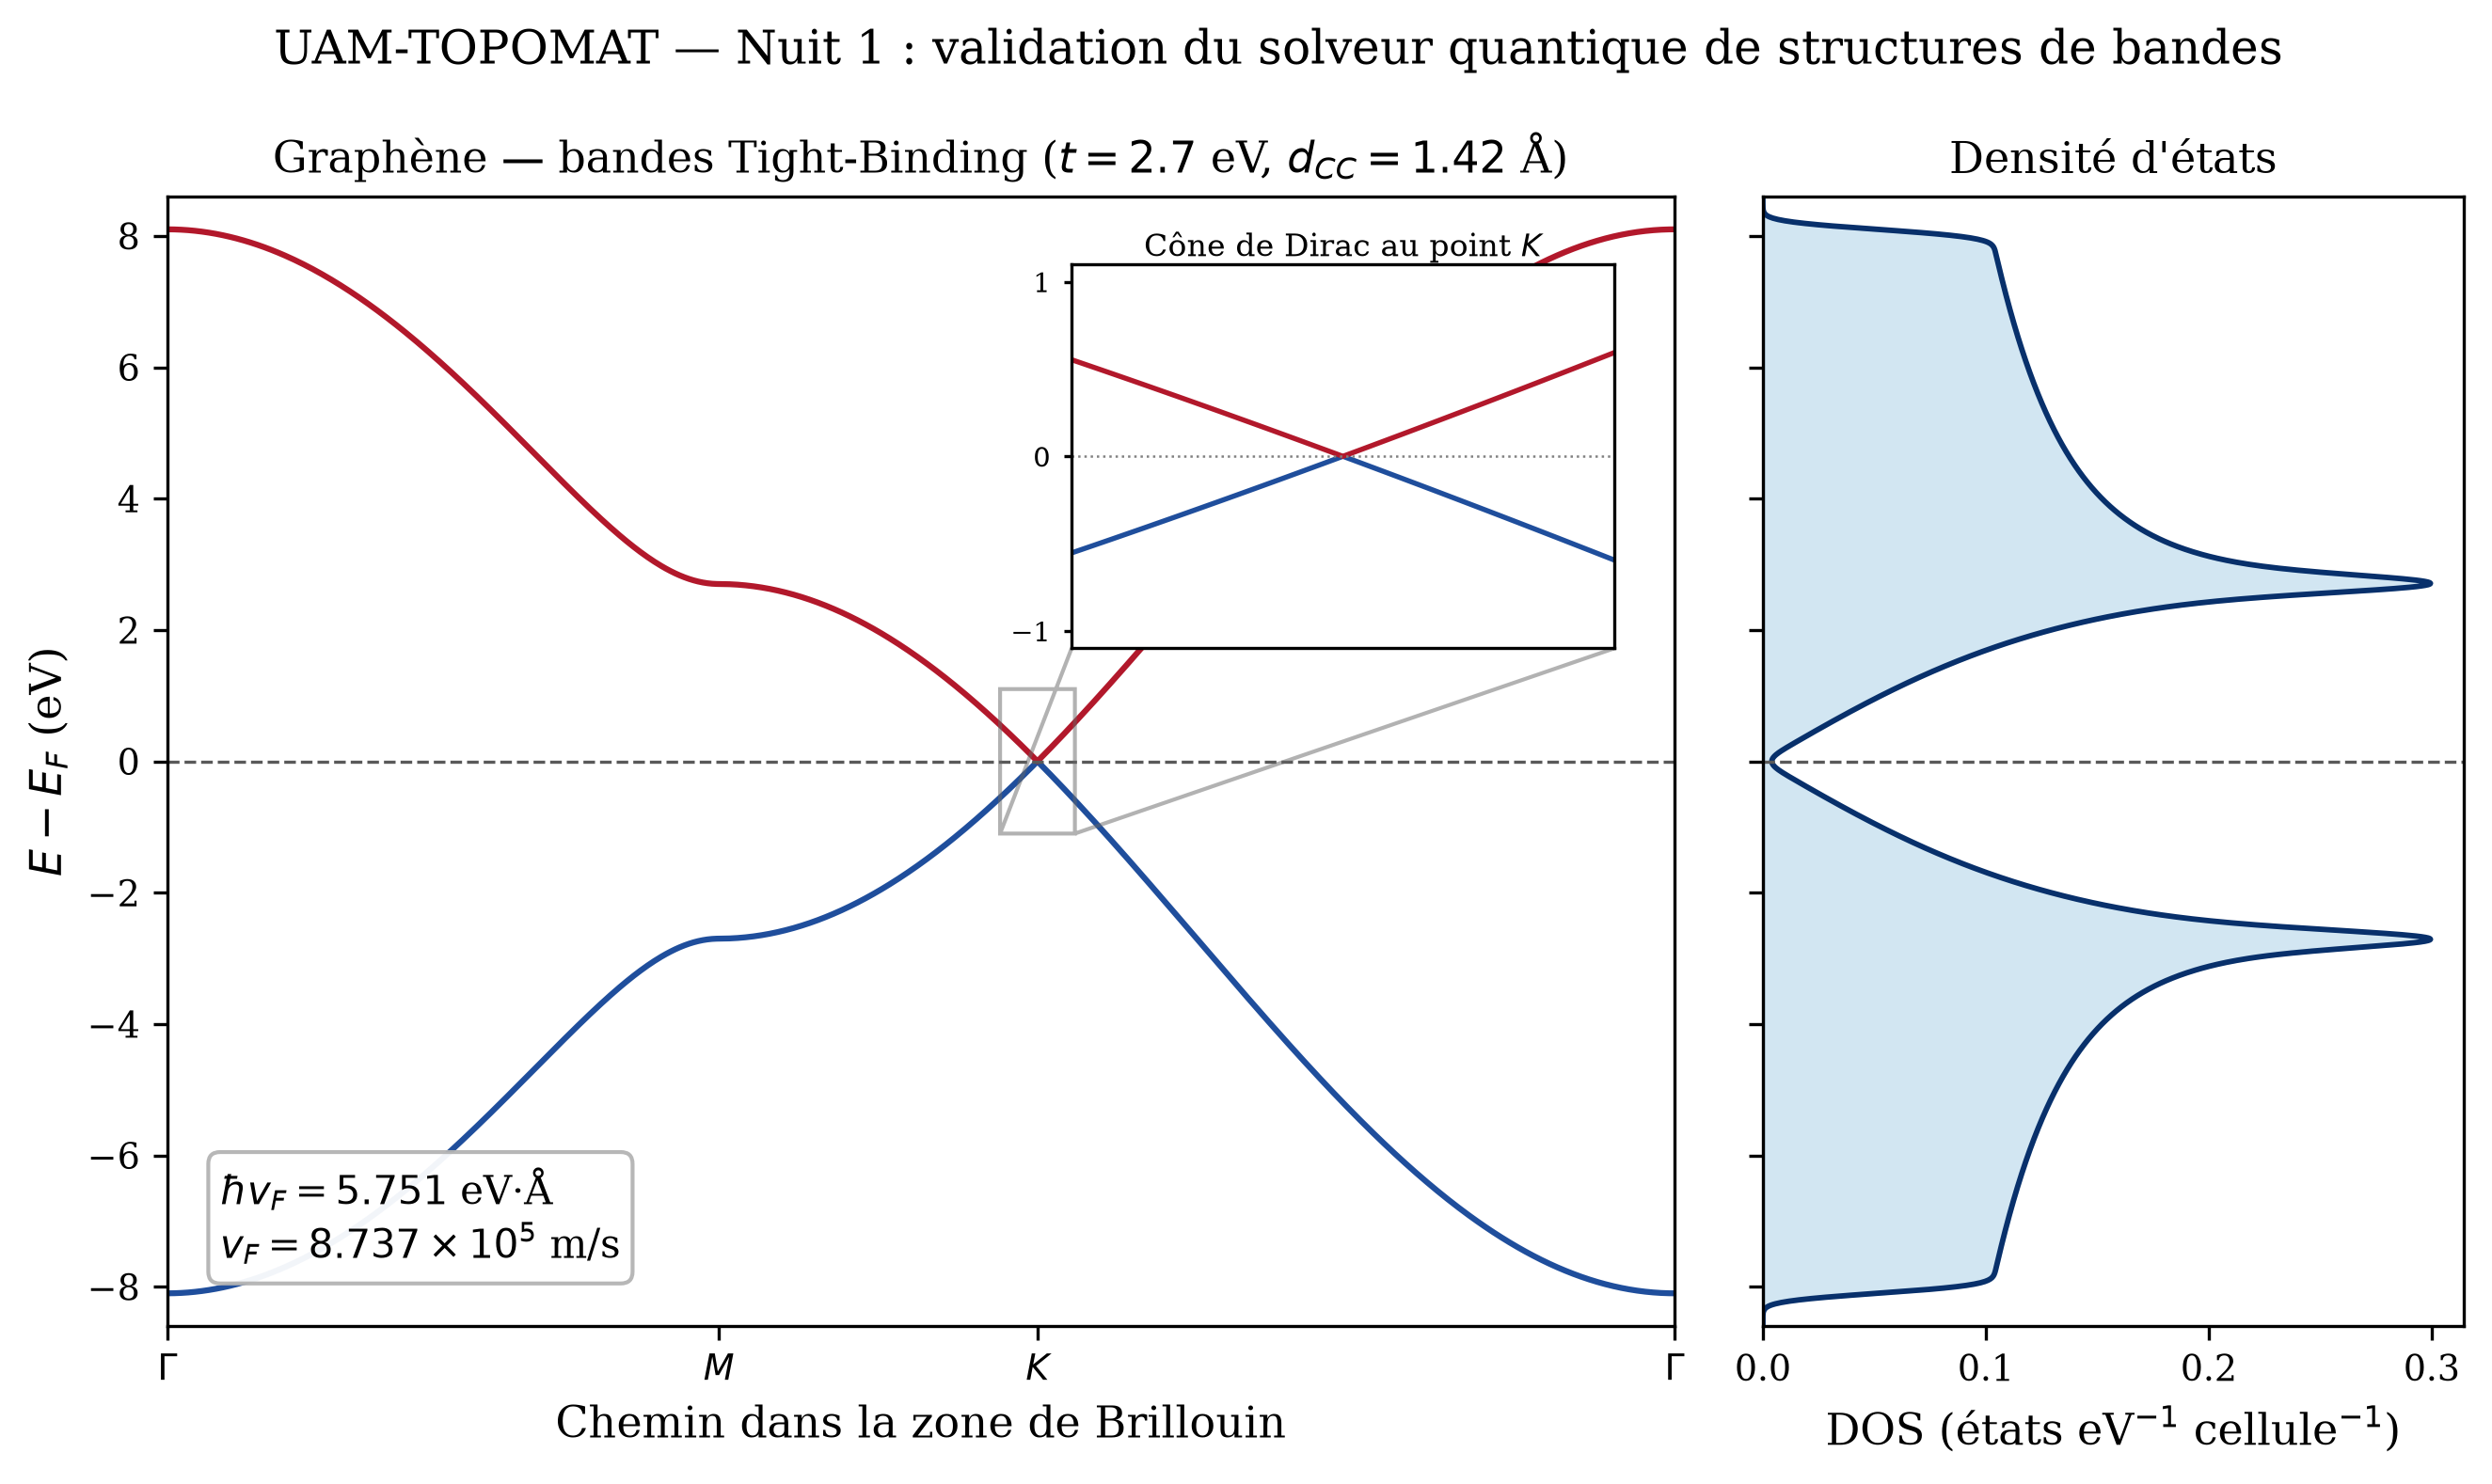
\includegraphics[width=0.92\linewidth]{night1_bands_dos.png}
\caption{Structure de bandes Tight-Binding et densité d'états (Nuit 1). Figure produite à 300~dpi.}
\end{figure}

\section{Conclusion et diffusion}
La chaîne UAM-TOPOMAT est désormais fermée : preuves formelles, certificats LaTeX, Top~10 et fiches techniques PDF. Les deux champions satisfont l'intégralité des bornes théoriques. Diffusion prévue : Twin Transition Summit, 1er décembre 2026 --- UAM / UFR STA / Cellule Physique.

\end{document}
